\chapter{Basics}

\section{Fundamental Theorem of Linear Algebra}

\begin{center}
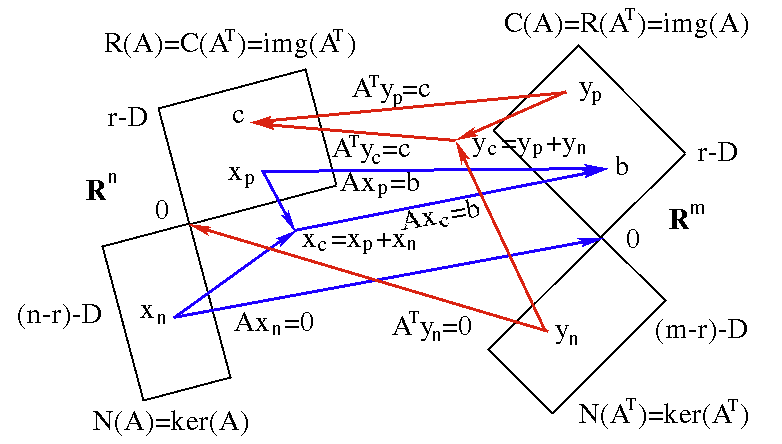
\includegraphics[width=\textwidth]{imgs/fund_theorem_lin_alg1.png}
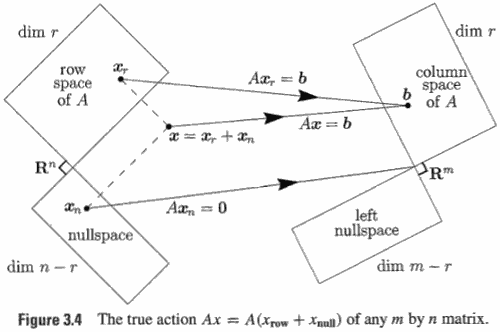
\includegraphics[width=\textwidth]{imgs/fund_theorem_lin_alg2.png}
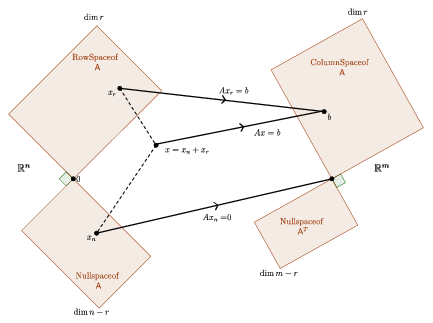
\includegraphics[width=\textwidth]{imgs/fund_theorem_lin_alg3.png}
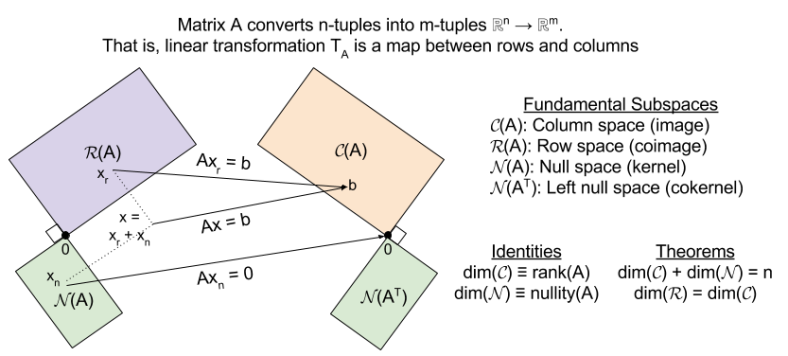
\includegraphics[width=\textwidth]{imgs/fund_theorem_lin_alg4.png}
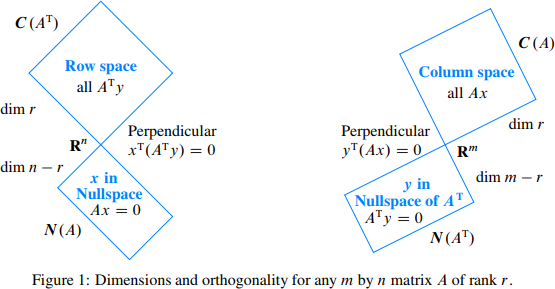
\includegraphics[width=\textwidth]{imgs/fund_theorem_lin_alg5.png}
\end{center}


\section{Matrix Properties}

\begin{align}
\mA(\mB+\mC) &=   \mA\mB+\mA\mC &\textrm{(left distributivity)}   \\
(\mB+\mC)\mA &=   \mB\mA+\mC\mA &\textrm{(right distributivity)}  \\
\mA\mB       &\ne \mB\mA        &\textrm{(in general)}            \\
(\mA\mB)\mC  &=   \mA(\mB\mC)   &\textrm{(associativity)}
\end{align}

\section{Matrix Multiplication}

\begin{equation}
(\mA\mB)_{kl} = \sum_m \mA_{km}\mB_{ml}~~~\mA\in\sR^{k,m},\mB\in\sR^{m,l}
\end{equation}


\section{Time Complexities}
\begin{center}
{\footnotesize\renewcommand{\arraystretch}{1.2}
\begin{tabular}{p{1.5cm}p{3cm}p{3cm}p{4cm}p{1cm}}
\textbf{Operation}             & \textbf{Input}                   & \textbf{Output}    & \textbf{Algorithm}                     & \textbf{Time}   \\ \hline
Matmult
    & $A,B\in n\times n$
    & $n \times n$
    & Schoolbook
    & $O(n^3)$
    \\ \hline

    &
    &
    & Strassen~\citep{Strassen1969}
    & $O(n^{2.807})$
    \\ \hline

    &
    &
    & Best
    & $O(n^\omega)$
    \\ \hline
Matmult
    & $A\in n\times m, B\in m\times p$
    & $n \times p$
    & Schoolbook
    & $O(nmp)$
    \\ \hline
Inversion
    & $A\in n\times n$
    & $n \times n$
    & Gauss--Jordan elimination
    & $O(n^3)$
    \\ \hline

    &
    &
    & Strassen~\citep{Strassen1969}
    & $O(n^{2.807})$
    \\ \hline

    &
    &
    & Best
    & $O(n^\omega)$
    \\ \hline
SVD
    & $A\in m\times n$
    & $m\times m, m\times n, n\times n$ \newline $m\times r, r\times r, n\times r$
    &
    & $O(mn^2)$ \newline \hbox{$(m\ge n)$} \\ \hline
Determinant
    & $A\in n\times n$
    & Scalar
    & Laplace expansion
    & $O(n!)$         \\ \hline

    &
    &
    & Division-free~\citep{Rote2001}
    & $O(n!)$
    \\ \hline

    &
    &
    & LU decomposition
    & $O(n^3)$
    \\ \hline

    &
    &
    & Integer preserving~\citep{Bareiss1968}
    & $O(n^3)$
    \\ \hline
Back \newline substitution
    & $A$ triangular
    & $n$ solutions
    & Back substitution
    & $O(n^2)$
    \\ \hline
\end{tabular}
}
\end{center}

\subsubsection{A comment on $\omega$}

The lower bound on matmult time complexity is $O(n^\omega)$, where $\omega$ is an unknown constant bounded by $2\le\omega\le2.373$. Algorithms achieving lower values of $\omega$ tend to be less efficient in practice for all but the largest matrices. Of the algorithm with times of less than $O(n^3)$, only the Strassen algorithm has seen serious attempts at optimized implementation. Most matmult implementations use highly optimized variants of the standard $O(n^3)$ algorithm. At this point, memory and bus speeds dominate the performance of implementations, so simple Big-O notation cannot be used to reliably compare matmult performances.

\begin{center}
\begin{tabular}{lll}
\textbf{Name}           & \textbf{Year} & $\omega$  \\
Standard                & -             & 3         \\
\citet{Strassen1969}    & 1969          & 2.807     \\
\citet{Pan1978}         & 1978          & 2.796     \\
\citet{Bini1979}        & 1979          & 2.78      \\
\citet{Schonhage1981}   & 1981          & 2.548     \\
\citet{Schonhage1981}   & 1981          & 2.522     \\
\citet{Romani1982}      & 1982          & 2.517     \\
\citet{Coppersmith1982} & 1982          & 2.496     \\
\citet{Strassen1986}    & 1986          & 2.479     \\
\citet{Copper1990}      & 1990          & 2.376     \\
\citet{Williams2012}    & 2012          & 2.37294   \\
\citet{LeGall2014}      & 2014          & 2.3728639 \\
\citet{Williams2012}    & 2012          & 2.3727    \\
\end{tabular}
\end{center}